\documentclass[11pt]{article}

\usepackage[margin=1in]{geometry}
\usepackage{amsmath,amssymb,amsthm,mathtools}
\usepackage{graphicx}
\usepackage{hyperref}
\usepackage{xcolor}

\hypersetup{
  colorlinks=true,
  linkcolor=blue!60!black,
  citecolor=blue!60!black,
  urlcolor=blue!60!black
}

\newtheorem{lemma}{Lemma}
\newcommand{\R}{\mathbb{R}}
\newcommand{\N}{\mathbb{N}}
\newcommand{\E}{\mathbb{E}}
\newcommand{\Pp}{\mathbb{P}}

\title{Duality in Mathematics}
\author{Zachary McNulty}
\date{}

\begin{document}
\maketitle

In convex optimization, one often sees references to \emph{dual problems},
which give an equivalent yet distinct viewpoint on the same optimization
problem. Lagrangian and Kantorovich duality are two classical examples, which
we discuss below. In this short note, we explore the general notion of duality:
how it arises, why it is so natural, and what we can do with it.

Below, let $V$ be an arbitrary normed real vector space, and let $V^*$ denote
its dual space: the space of linear functionals on $V$. For our purposes, we
will think of $V=\R^d$, so that we can ignore some necessary regularity
assumptions that appear in infinite dimensions. Even though $\R^d$ is
self-dual, it is convenient to denote $V$ and $V^*$ separately.

The discussion of perturbation duality in
\href{https://math.stackexchange.com/questions/223235/please-explain-the-intuition-behind-the-dual-problem-in-optimization}{this
Math Stack Exchange post} is quite informative. These
\href{https://www.mit.edu/~gfarina/2025/67220s25_L03_more_on_normal_cones/L03.pdf}{course
notes} are also useful for understanding normal cones in Lagrangian duality.

\section{What Is Duality in Mathematics?}

Duality is a somewhat ill-defined principle in mathematics, but it generally
describes the idea that problems in one setting can often be translated to
problems in another setting in a one-to-one fashion, often in the form of an
\emph{involution}. This becomes particularly useful when the dual space has
some structure that the primal space lacks, allowing us to apply a different
set of tools to study the same underlying problem.

We begin with some simple examples and move toward more sophisticated
applications. Some of the more complicated examples can be skipped on a first
reading and revisited after the rest of the note.

\subsection{Set Complements}

Given a subset $A\subseteq S$, properties of $A$ can often be framed in terms
of its complement $A^c$. For example, in topology a set $A$ is closed if and
only if $A^c$ is open. This allows us to state many topological properties in
terms of either open sets or closed sets:

\begin{itemize}
  \item \emph{Continuity}: the preimage of every open set is open if and only
  if the preimage of every closed set is closed.
  \item \emph{Compactness}: an open cover $\{U_\alpha\}$ of $K$ has a finite
  subcover if and only if $K^c$ contains a finite intersection of the
  $U_\alpha^c$.
  \item \emph{Closure and interior}: $\operatorname{Int}(S)^c=\overline{S^c}$.
  \item \emph{Denseness}: every open set $U\subseteq X$ intersects $S$ if and
  only if $\overline S=X$.
  \item \emph{Hausdorffness}: every $x,y$ can be separated by open sets if and
  only if $\{x\}=\bigcap_{F\in C_x}F$, where
  $C_x=\{F\text{ closed}:x\in F\}$.
\end{itemize}

The map $A\mapsto A^c$ is an involution, and $A\subseteq B$ implies
$A^c\supseteq B^c$, so it reverses the natural inclusion order.

\subsection{Dual Cones}

Given $C\subseteq V$, define its \emph{dual cone} by
\[
  C^*:=\{v\in V^*: \langle v,x\rangle\geq 0\quad\text{for every }x\in C\},
\]
where $\langle v,x\rangle:=v(x)$ applies the dual functional to $x$. As in the
previous example, this duality reverses the natural inclusion order. However,
it is an involution only under suitable conditions on $C$.

\begin{figure}[ht]
  \centering
  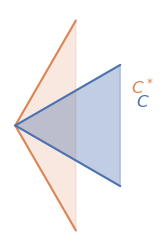
\includegraphics[height=2.2in]{images/dual-cones.png}
  \caption{A cone and its dual cone.}
\end{figure}

\subsection{Dual Vector Spaces}

Probably the most iconic instance of duality is the dual of a vector space.
Given $V$, define $V^*$ as the set of all linear functionals
$\phi:V\to\R$. This duality is useful because $V^*$ is a space of
\emph{functions}, allowing us to apply a wide range of tools from functional
analysis. Linear maps $T:V\to W$ induce linear maps $T^*:W^*\to V^*$ via
$T^*(\phi):=\phi\circ T$. Notice that the direction of the arrow is reversed.

\subsection{Dual Graphs}

Any planar graph $G$ divides two-dimensional space into a collection of closed
regions, called \emph{faces}, together with a possibly unbounded exterior
region. We define another graph $G^*$ by adding one vertex for each face and
an edge between two vertices whenever their corresponding faces are adjacent
along an edge of $G$. Generally, $G^*$ depends on the chosen planar embedding,
but many of its properties are invariant under the embedding. Here duality is
a genuine involution in the sense that, once an embedding is fixed,
$G^{**}\cong G$.

The graph $G^*$ encodes connectivity in the original graph. One manifestation
of this is the relationship between cycles and cut sets. A cut set is a subset
of the edges of $G$ obtained by partitioning its vertices into two parts and
collecting the edges between those parts. Since there is a bijection between
the edges of $G$ and $G^*$, a cycle in $G$ induces a cut set in $G^*$,
partitioning the dual vertices into the faces inside and outside the cycle.
Thus minimal cycles in $G$ correspond to minimal cut sets in $G^*$, and vice
versa.

One classical example comes from bond percolation on the lattice $\mathbb Z^2$.
Suppose each edge is independently retained with probability $p$ to form a
random graph $G$. We are interested in the probability that there is a path in
$G$ from the origin to infinity. Such a path exists if and only if the dual
graph contains no closed dual cycle separating the origin from infinity.

\begin{lemma}
There exists $p<1$ such that $\Pp(0\leftrightarrow\infty)>0$.
\end{lemma}

\begin{proof}
This is a classical Peierls-style argument. A given dual path $\gamma$ of
length $n$ is closed with probability $(1-p)^n$. Since there are at most three
non-backtracking choices at every step, there are at most $3^n$ candidate paths
of length $n$. If the origin is not connected to infinity, some closed dual
cycle must surround it. Therefore, by the union bound,
\[
  \Pp(0\not\leftrightarrow\infty)
  \leq \sum_{n\geq4}3^n(1-p)^n
  =\frac{3^4(1-p)^4}{3p-2},
\]
which is less than one when $p$ is sufficiently close to one.
\end{proof}

\subsection{Duality in Population Genetics}

In population genetics, we study how the genetic makeup of a population
evolves over time due to randomness in reproduction, natural selection, and
mutation. In the simplest case, suppose a gene has two alleles, $a$ and $A$.
The same process can often be viewed under two lenses: forward in time, by
tracking how alleles are passed from one generation to the next, or backward in
time, by taking present-day individuals and tracing their ancestral lineages.

The Wright--Fisher model assumes that $N$ individuals in each generation
independently sample a parent from the previous generation and inherit its
allele. If $X_t$ is the number of individuals carrying $A$ at generation $t$,
then
\[
  X_{t+1}\sim\operatorname{Binomial}(N,p_t),
  \qquad p_t:=\frac{X_t}{N}.
\]
To model selection, introduce a bias $\alpha\geq0$ favoring $A$ and set
\[
  X_{t+1}\sim\operatorname{Binomial}(N,p_t),
  \qquad p_t:=\frac{(1+\alpha)X_t}{N+\alpha X_t}.
\]
After taking $N\to\infty$ and speeding up time, one obtains the Wright--Fisher
diffusion
\[
  dp_t=\alpha p_t(1-p_t)\,dt+\sqrt{p_t(1-p_t)}\,dW_t.
\]
Both the drift in allele frequency and the random fluctuations depend on
$p(1-p)$, which measures, in a sense, the distance from fixation.

The backward-time dynamics can be simpler. We seek a function $f(p,n)$ relating
the forward and backward processes such that
\[
  \frac{d}{du}\E[f(p(u),n(t-u))]=0,
  \qquad 0\leq u\leq t,
\]
and hence
\[
  \E[f(p(t),n(0))]=\E[f(p(0),n(t))].
\]
If $L$ and $G$ are the generators of $p_t$ and $n_t$, respectively, this is
suggested by the generator relationship
\[
  Lf_n(p)=Gf_p(n),
  \qquad f_n(p)=f_p(n):=f(n,p).
\]

In the neutral case $\alpha=0$, $p_t$ has generator
\[
  Lg(p)=\frac{p(1-p)}{2}g''(p).
\]
The corresponding backward-time process is Kingman's coalescent. Its number of
remaining ancestral lineages $n(t)$ is a pure-death process on $\N$ with
generator
\[
  Gg(n)=-\binom{n}{2}\bigl(g(n)-g(n-1)\bigr).
\]
These generators suggest $f(n,p)=p^n$, because
\[
  Lf_n(p)=Gf_p(n)=-\binom{n}{2}(p^n-p^{n-1}).
\]
This gives the duality relationship
\[
  \E[p(t)^{n(0)}]=\E[p(0)^{n(t)}].
\]

Both sides give the probability that a sample of $n(0)$ present-day
individuals all carry $A$. The left side samples directly from the present
population. The right side evolves the sample backward to its ancestral
lineages and asks for the probability that each ancestor carried $A$.

This duality also determines the fixation probability. Since $n(t)=1$ almost
surely as $t\to\infty$ in Kingman's coalescent, the right-hand expectation
converges to $p(0)$. Consequently, the probability that $A$ ultimately fixes is
$p(0)$, a conclusion that is much easier to obtain from the dual process than
directly from the diffusion.

\section{Convex Sets and Supporting Hyperplanes}

A set $X\subseteq V$ is \emph{convex} if it is closed under affine
combinations:
\[
  x,y\in X\quad\Longrightarrow\quad
  \lambda x+(1-\lambda)y\in X
  \quad\text{for every }\lambda\in[0,1].
\]
Given $X$, a \emph{supporting hyperplane} is a hyperplane that intersects
$\partial X$ and leaves all of $X$ in one of its two closed half-spaces. More
formally, $H=\{x:\ell(x)=b\}$ for $\ell\in V^*$ and $b\in\R$ supports $X$ if
\[
  \ell(x)\leq b\quad\text{for every }x\in X,
  \qquad
  \ell(x_0)=b\quad\text{for some }x_0\in X.
\]
Such a hyperplane is tangent, in a generalized sense, to the boundary of $X$.

A fundamental result in convex analysis says that if $X$ is closed and convex
in a suitably nice topological vector space, then each boundary point admits a
supporting hyperplane. In particular, $X$ is the intersection of all closed
half-spaces that contain it. Since these half-spaces are defined by dual
elements $\ell\in V^*$, this creates a natural relationship between a convex
set and the dual space.

The \emph{support function} $\sigma_X:V^*\to\R\cup\{+\infty\}$ is
\[
  \sigma_X(\ell):=\sup_{x\in X}\ell(x).
\]
It encodes the supporting level associated with each dual direction, and
\[
  X=\bigcap_{\ell\in V^*}
  \{x\in V:\ell(x)\leq\sigma_X(\ell)\}.
\]
Thus convex analysis contains a duality between convex sets and linear
functionals, with $\sigma_X$ encoding the relationship.

\section{Convex Conjugates}

A set $X$ is closed and convex if and only if its indicator function
$\iota_X:V\to\overline\R$,
\[
  \iota_X(x):=
  \begin{cases}
    0,&x\in X,\\
    +\infty,&x\notin X,
  \end{cases}
\]
is a closed convex function. The support function can then be written as
\[
  \sigma_X(\ell)=\sup_{x\in V}\{\ell(x)-\iota_X(x)\}.
\]
Here $\iota_X$ encodes the hard constraint $x\in X$, while $\sigma_X(\ell)$
records the maximal value of the objective $\ell$ subject to that constraint.
For example, if $X=\{x:\lVert x\rVert_2\leq1\}$ is the Euclidean unit ball,
then
\[
  \sigma_X(\ell)=\sup_{x\in X}\ell^\top x=\lVert\ell\rVert_2.
\]

For a general convex function $\phi:V\to\overline\R$, define its
\emph{convex conjugate} $\phi^*:V^*\to\overline\R$ by
\[
  \phi^*(\ell):=\sup_{x\in V}\{\ell(x)-\phi(x)\}.
\]
Instead of imposing a hard constraint, we introduce a convex potential
$\phi$. The conjugate records the optimal balance between maximizing the
linear objective $\ell$ and minimizing the potential $\phi$.

There is also a geometric interpretation. A function $f:V\to\R$ is convex if
and only if its epigraph
\[
  \operatorname{epi}(f):=\{(x,y)\in V\times\R:y\geq f(x)\}
\]
is convex. The convex conjugate is defined so that
\[
  \langle\ell,x\rangle-f^*(\ell)\leq f(x)
  \qquad\text{for every }x\in V.
\]
It therefore selects the highest affine function of slope $\ell$ that lies
entirely below $f$. In one dimension these supporting hyperplanes are simply
supporting lines.

\begin{figure}[ht]
  \centering
  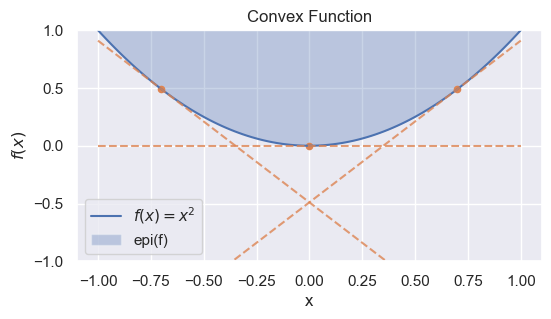
\includegraphics[width=.72\textwidth]{images/convex-conjugate.png}
  \caption{Supporting lines below the convex function $f(x)=x^2$.}
\end{figure}

\section{Duality in Convex Analysis}

Suppose we want to solve the convex optimization problem
\[
  \min_x f(x)
  \qquad\text{subject to}\qquad
  g_i(x)\leq0,\quad i\in[m],
\]
where $f$ and the $g_i$ are convex. For simplicity, assume all these functions
are differentiable.

\subsection{Duality Through Perturbation}

\emph{This section remains to be completed.}

\subsection{Strong Duality}

\emph{This section remains to be completed.}

\section{Examples of Duality in Optimization}

\subsection{Lagrangian Duality}

Lagrangian duality begins with the observation that if $x^*$ minimizes the
optimization problem, then
\[
  \langle-\nabla f(x^*),v\rangle\leq0
\]
for every feasible direction $v$: there is no direction in which we can both
remain feasible and decrease the objective.

First consider a single equality constraint,
\[
  \min_x f(x)\qquad\text{subject to}\qquad g(x)=0.
\]
At a point $x$, $\nabla g(x)$ is perpendicular to the level set $\{g=0\}$,
so the first-order optimality condition becomes
\[
  \nabla f(x)=\lambda\nabla g(x),\qquad\lambda\in\R.
\]
With several equality constraints,
\[
  \min_x f(x)\qquad\text{subject to}\qquad
  g_i(x)=0,\quad i\in[m],
\]
the feasible directions are perpendicular to every $\nabla g_i(x)$. Thus
\[
  \nabla f(x)=\sum_{i=1}^m\lambda_i\nabla g_i(x),
  \qquad\lambda_i\in\R.
\]

Now consider inequality constraints $g_i(x)\leq0$. At $x^*$, a constraint is
\emph{inactive} when $g_i(x^*)<0$ and \emph{active} when $g_i(x^*)=0$.
Writing $A(x)=\{i:g_i(x)=0\}$, the local feasible directions are
\[
  F_x=\{v\in\R^n:\langle v,\nabla g_i(x^*)\rangle\leq0
  \text{ for every }i\in A(x^*)\}.
\]
The optimality condition can therefore be expressed as
\[
  -\nabla f(x^*)=
  \sum_{i\in A(x^*)}\lambda_i\nabla g_i(x^*),
  \qquad\lambda_i\geq0.
\]
Complementary slackness lets us avoid naming the active set explicitly:
\[
  -\nabla f(x^*)=\sum_{i=1}^m\lambda_i\nabla g_i(x^*),
  \qquad
  \lambda_i g_i(x^*)=0,
  \qquad\lambda_i\geq0.
\]

These observations are encoded in the \emph{Lagrangian}
\[
  L(x,\lambda):=f(x)+\sum_{i=1}^m\lambda_i g_i(x),
  \qquad\lambda_i\geq0.
\]
Stationarity in $x$ gives
\[
  \nabla_xL(x,\lambda)
  =\nabla f(x)+\sum_{i=1}^m\lambda_i\nabla g_i(x)=0.
\]
For fixed $\lambda$, the Lagrangian can also be viewed as a soft version of the
original constrained problem. If $x$ is feasible, then
$L(x,\lambda)\leq f(x)$ for every $\lambda\geq0$. Define the dual objective
\[
  h(\lambda):=\inf_xL(x,\lambda).
\]
If $x^*$ solves the primal problem, then
\[
  h(\lambda)
  \leq\inf_{x\text{ feasible}}L(x,\lambda)
  \leq f(x^*).
\]
This motivates the dual problem
\[
  \max_{\lambda\geq0}h(\lambda).
\]
The inequality $h(\lambda^*)\leq f(x^*)$ is \emph{weak duality}. Under
additional assumptions, such as Slater's condition, equality holds and we
obtain \emph{strong duality}:
\[
  \max_{\lambda\geq0}h(\lambda)
  =\min_{x\text{ feasible}}f(x).
\]

\subsubsection{Application: Duality in Linear Programming}

A linear program is a convex optimization problem whose objective and
constraints are linear:
\[
  \min_x c^\top x\qquad\text{subject to}\qquad Ax\leq b.
\]
Its Lagrangian is
\[
  L(x,\lambda)=c^\top x+\lambda^\top(Ax-b),
  \qquad\lambda\geq0.
\]
Stationarity enforces the dual constraint
\[
  \nabla_xL(x,\lambda)=0
  \quad\Longrightarrow\quad
  A^\top\lambda=-c.
\]
Under this constraint,
\[
  h(\lambda):=\inf_xL(x,\lambda)=-\lambda^\top b.
\]
Hence the dual problem is
\[
  \max_\lambda-\lambda^\top b
  \qquad\text{subject to}\qquad
  A^\top\lambda=-c,
  \quad\lambda\geq0.
\]

\subsection{Kantorovich Duality}

\emph{To be completed: interpret the functions $\phi$ and $\psi$ in the
Kantorovich dual problem.}

\end{document}
